\documentclass{article}
\usepackage{xcolor}
\usepackage{titleps}
\usepackage[letterpaper, margin=0.95in]{geometry}
\usepackage{url}
\usepackage{amsmath}
\usepackage{amssymb}
\usepackage{wrapfig}
\usepackage{float}
\usepackage{mathtools}
\usepackage{enumitem}
\usepackage{tabu}
\usepackage{parskip}
\usepackage{natbib}
\usepackage{listings}
\usepackage{tikz}

\newcommand{\xb}{\mathbf{x}}
\newcommand{\yb}{\mathbf{y}}
\newcommand{\wb}{\mathbf{w}}
\newcommand{\Xb}{\mathbf{X}}
\newcommand{\Yb}{\mathbf{Y}}
\newcommand{\tr}{^T}
\newcommand{\hb}{\mathbf{h}}
\newcommand{\Hb}{\mathbf{H}}

\DeclareFontShape{OT1}{cmtt}{bx}{n}{<5><6><7><8><9><10><10.95><12><14.4><17.28><20.74><24.88>cmttb10}{}


\usepackage{forest}

\usepackage{hyperref}
\usepackage[color=red]{todonotes}
\usepackage{forest}
\definecolor{light-yellow}{HTML}{FFE5CC}

\usepackage{cleveref}

\newpagestyle{ruled}
{\sethead{Berkeley CS 285}{Deep Reinforcement Learning, Decision Making, and Control}{Fall 2023}\headrule
    \setfoot{}{}{}}
\pagestyle{ruled}

\renewcommand\makeheadrule{\color{black}\rule[-.75\baselineskip]{\linewidth}{0.4pt}}
\renewcommand*\footnoterule{}

\usepackage{subcaption} % Add this line

\begin{document}
\newcommand*{\MYSOLUTION}[0]{\textcolor{red}{\textbf{My Solutions: }}}
\lstset{basicstyle = \ttfamily,columns=fullflexible,
backgroundcolor = \color{light-yellow}
}

\begin{centering}
        {\Large [SOLUTION TEMPLATE] Assignment 2: Policy Gradients} \\
        \vspace{.25cm}
        \textbf{Due September 25, 11:59 pm} \\
\end{centering}

\setcounter{section}{2}
\section{Policy Gradients}
\begin{itemize}
\item Create two graphs:
\begin{itemize}
\item In the first graph, compare the learning curves (average return vs. number of environment steps) for the experiments prefixed with \verb|cartpole|. (The small batch experiments.)
\item In the second graph, compare the learning curves for the experiments prefixed with \verb|cartpole_lb|. (The large batch experiments.)
\end{itemize}
\textbf{For all plots in this assignment, the $x$-axis should be number of environment steps, logged as} \verb|Train_EnvstepsSoFar| \textbf{(\textit{not} number of policy gradient iterations).}

\MYSOLUTION

\begin{figure}[h]
        \centering
        \begin{subfigure}{0.45\textwidth}
                \centering
                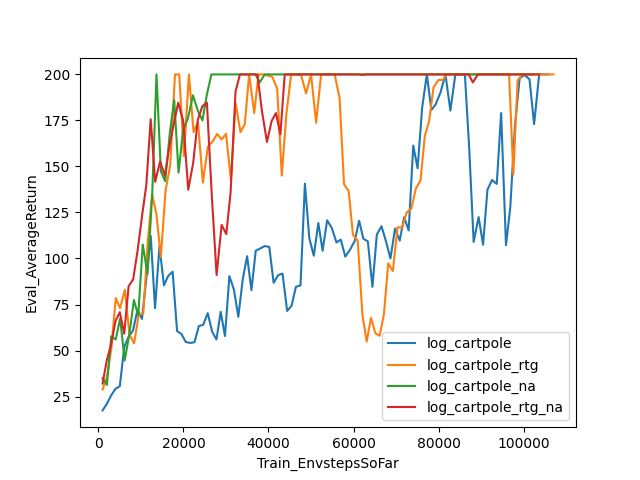
\includegraphics[width=\linewidth]{./report/assets/all_E1-1.png} % Replace with your first graph
                \caption{Small batch experiments}
                \label{fig:graph1}
        \end{subfigure}
        \hfill
        \begin{subfigure}{0.45\textwidth}
                \centering
                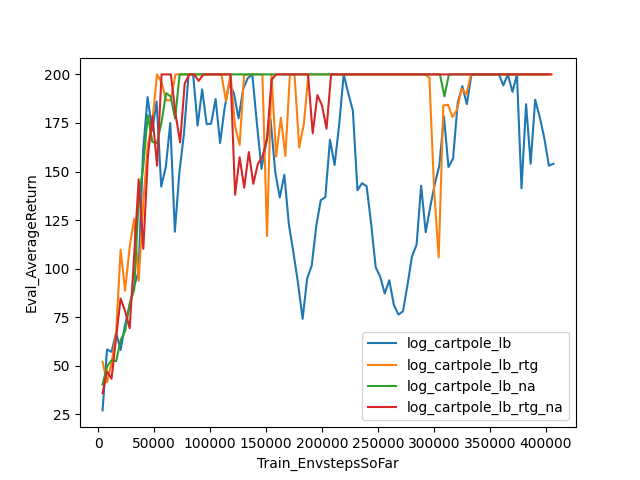
\includegraphics[width=\linewidth]{./report/assets/all_E1-2.png} % Replace with your second graph
                \caption{Large batch experiments}
                \label{fig:graph2}
        \end{subfigure}
        \caption{Learning curves for different experiments}
        \label{fig:graphs}
\end{figure}


\item Answer the following questions briefly: 
\begin{itemize}
\item Which value estimator has better performance without advantage normalization: the trajectory-centric one, or the one using reward-to-go?
\item \MYSOLUTION Without advantage normalization, using reward-to-go is better; with advantage normalization, the two ways have similar performance.
\item Did advantage normalization help?
\item \MYSOLUTION Yes.
\item Did the batch size make an impact?
\item \MYSOLUTION Yes, the large batch size has better performance.
\end{itemize}
\item Provide the exact command line configurations (or \texttt{\#@params} settings in Colab) you used to run your experiments, including any parameters changed from their defaults.

\MYSOLUTION 
\begin{verbatim}
 python cs285/scripts/run_hw2.py --env_name CartPole-v0 -n 100 -b 1000 \
        --exp_name cartpole \
        > log_cartpole.log
\end{verbatim}

I haven't change any parameters from their defaults.

\end{itemize}

\newpage\section{Neural Network Baseline}
\begin{itemize}
        \item Plot a learning curve for the baseline loss.

\MYSOLUTION

\begin{figure}[h]
        \centering
        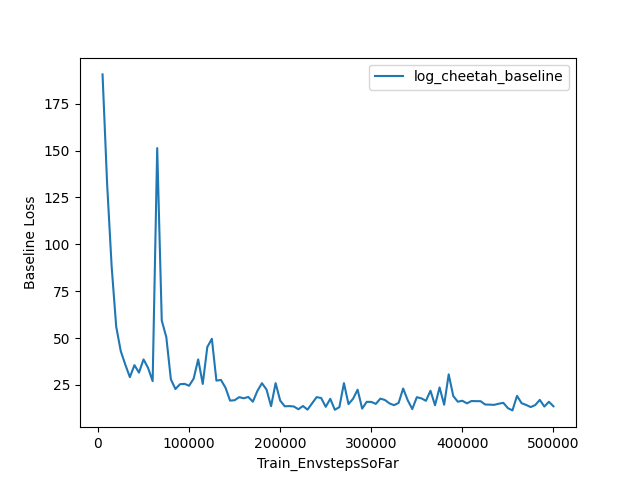
\includegraphics[width=0.5\linewidth]{./report/assets/all_E2_baseline.png} % Replace with your graph
        \caption{Learning curve for the baseline loss}
        \label{fig:E2_baseline_loss}
\end{figure}
        \item Plot a learning curve for the eval return. You should expect to achieve an average return over 300 for the baselined version.

\MYSOLUTION

\begin{figure}[h]
        \centering
        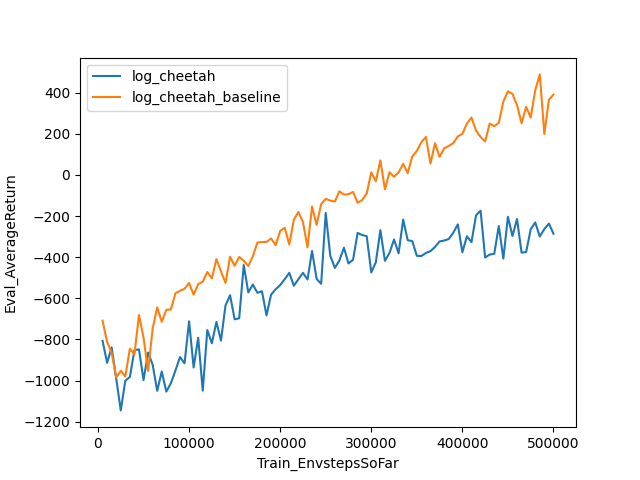
\includegraphics[width=0.5\linewidth]{./report/assets/all_E2.png} % Replace with your graph
        \caption{Learning curve for eval return}
        \label{fig:eval_return_E2}
\end{figure}

        \item Run another experiment with a decreased number of baseline gradient steps (\verb|-bgs|) and/or baseline learning rate (\verb|-blr|). How does this affect (a) the baseline learning curve and (b) the performance of the policy?

\MYSOLUTION

\begin{figure}[H]
        \centering
        \begin{subfigure}{0.45\textwidth}
                \centering
                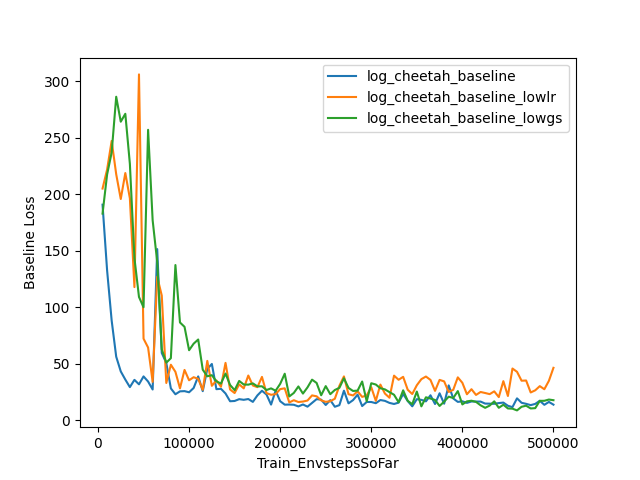
\includegraphics[width=\linewidth]{./report/assets/all_E2_baseline_hyperparam.png} % Replace with your first graph
                \caption{Change of baseline loss}
                \label{fig:E2-baseline-loss}
        \end{subfigure}
        \hfill
        \begin{subfigure}{0.45\textwidth}
                \centering
                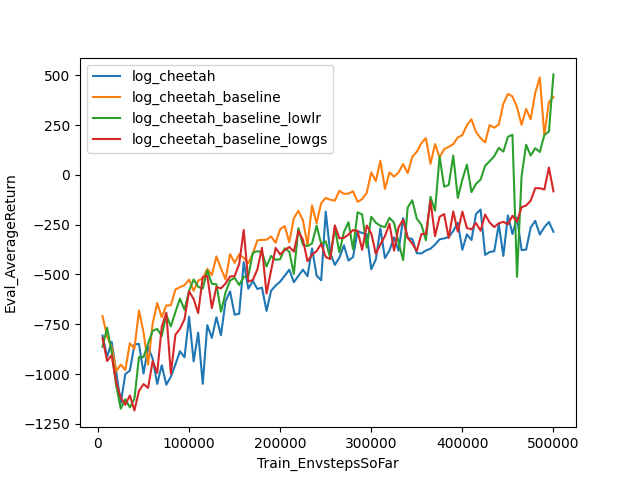
\includegraphics[width=\linewidth]{./report/assets/all_E2_comp.png}
                % Replace with your second graph
                \caption{Change of policy performance}
                \label{fig:E2-policy-performance}
        \end{subfigure}
        \caption{Learning curves for different experiments}
        \label{fig:E2-change-hyperparam}
\end{figure}

From the figures, we can see that the decreasing the learning rate of the baseline from 0.01 to 0.004 doesn't matter much to the final performance of the policy, but it harms the final baseline loss. On the other hand, decreasing the number of baseline gradient steps from 5 to 2 doesn't affect the final baseline loss much (only the convergence rate becomes slower), but it the performance of the policy is strongly harmed.

        \item \textbf{Optional:} Add \verb|-na| back to see how much it improves things. Also, set \verb|video_log_freq 10|, then open TensorBoard and go to the ``Images'' tab to see some videos of your HalfCheetah walking along!
\end{itemize}

\newpage\section{Generalized Advantage Estimation}
\begin{itemize}
        \item Provide a single plot with the learning curves for the \verb|LunarLander-v2| experiments that you tried. Describe in words how $\lambda$ affected task performance. The run with the best performance should achieve an average score close to 200 (180+).
        \item Consider the parameter $\lambda$. What does $\lambda = 0$ correspond to? What about $\lambda = 1$? Relate this to the task performance in \verb|LunarLander-v2| in one or two sentences.
\end{itemize}

\newpage\section{Hyperparameter Tuning}
\begin{enumerate}
        \item Provide a set of hyperparameters that achieve high return on \verb|InvertedPendulum-v4| in as few environment steps as possible.
        \item Show learning curves for the average returns with your hyperparameters and with the default settings, with environment steps on the $x$-axis. Returns should be averaged over 5 seeds.
\end{enumerate}

\newpage\section{(Extra Credit) Humanoid}
\begin{enumerate}
        \item Plot a learning curve for the Humanoid-v4 environment. You should expect to achieve an average return of at least 600 by the end of training. Discuss what changes, if any, you made to complete this problem (for example: optimizations to the original code, hyperparameter changes, algorithmic changes).
\end{enumerate}



\setcounter{section}{8}
\newpage\section{Survey}
\label{sec:survey}
Please estimate, in minutes, for each problem, how much time you spent (a) writing code and (b) waiting for the results. This will help us calibrate the difficulty for future homeworks. 
\begin{itemize}
        \item \textbf{Policy Gradients:}
        \item \textbf{Neural Network Baseline:}
        \item \textbf{Generalized Advantage Estimation:}
        \item \textbf{Hyperparameters and Sample Efficiency:}
        \item \textbf{Humanoid:}
        \item \textbf{Humanoid:}
        \item \textbf{Analysis -- applying policy gradients:}
        \item \textbf{Analysis -- PG variance:}
        \item \textbf{Analysis -- return-to-go:}
        \item \textbf{Analysis -- importance sampling:}
\end{itemize}

\end{document}
